%
% File hicss51.tex
%
% Contact: Holm Smidt, hsmidt@hawaii.edu
%%
%%
%% Based on the style files for ACL 2015 by 
%% car@ir.hit.edu.cn, gdzhou@suda.edu.cn


\documentclass[10pt]{article}
\usepackage[letterpaper]{geometry}
\usepackage{hicss51}
\usepackage{times}
\usepackage[none]{hyphenat}
\usepackage{url}
\usepackage{latexsym}
\usepackage{minted}
\usepackage{indentfirst}
\usepackage{graphicx}
\usepackage{datetime}
\usepackage{cite}
\usepackage[hyphens]{url}
\usepackage[hidelinks]{hyperref}
\usepackage{csquotes}
\usepackage{array}
\usepackage{multirow}
\usepackage{multicol}
\usepackage{pdflscape}
\usepackage{amsmath}
\usepackage{float}
\usepackage{afterpage}
\hypersetup{breaklinks=true}
\newcommand{\subparagraph}{}
\usepackage{titlesec}
\setcounter{secnumdepth}{4}
\graphicspath{{images/}}

\newcommand{\sansserifformat}[1]{\fontfamily{cmss}{ #1}}%
\usepackage{adjustbox}
\usepackage{array}
\usepackage{amssymb}% http://ctan.org/pkg/amssymb
\usepackage{pifont}% http://ctan.org/pkg/pifont
\newcommand{\cmark}{\ding{51}}%
\newcommand{\xmark}{\ding{55}}
%\setlength\titlebox{5cm}

% You can expand the titlebox if you need extra space
% to show all the authors. Please do not make the titlebox
% smaller than 5cm (the original size).


\title{Fighting XSS.\\
\large A Usability Evaluation of OWASP ESAPI Output Encoding}

%\author{First Author \\
%  Affiliation \\
%  {\underline{ email@domain}} \\\And
%  Second Author \\
%  Affiliation \\
%  {\underline{ email@domain} }\\\And 
%  Third Author \\
%  Affiliation \\
%  {\underline{email@domain}} \\}

\date{}

\begin{document}
\maketitle
\begin{abstract}
The abstract is to be in fully-justified italicized text, at the top of the left-hand column as it is here, below the author information. Use the word “Abstract” as the title, in 12-point Times, boldface type, centered relative to the column, initially capitalized. The abstract is to be in 10-point, single-spaced type, and up to 150 words in length. Leave two blank lines after the abstract, and then begin the main text. 

\end{abstract}

\section{Introduction}

2017 OWASP Top 10 \cite{owasp10application} listed Cross Site Scripting (XSS) as 1 of the 10 most critical security risks for web applications. XSS has been ranked among top 10 most critical security risks for web applications since the start of OWASP Top 10 project in 2010. According OWASP Top 10 2017 report \cite{owasp10application}, XSS has been the 2nd most prevalent security issue and it exists in 2/3 of web applications. 

XSS is a security vulnerability that allows attackers to inject client-side malicious scripts into web pages of the applications that will thereafter execute in other users web browsers when they access those web pages \cite{owasp10xss}. Attackers can use this vulnerability to do various malicious things such as stealing user's session cookies, hijacking user session and take over the account, installing Trojan horse programs in user computers, etc \cite{owasp10xss}.

Programmers can prevent their web applications from being vulnerable to XSS attacks by separating untrusted data from active browser content \cite{owasp10application}. One of the techniques of achieving this is encoding untrusted output data when loading them into browser content \cite{owasp10application, owasp10cheat}. However, most programmers who are involved in application development are not security experts and they are not capable of implementing such security techniques in their own \cite{wurster}. Therefore, security experts have developed these functionalities so that non-expert programmers can use those functionalities in their applications via Application Programming Interfaces (APIs). There are several APIs that implement output encoding functionalities that programmers can use to protect their applications from being vulnerable to XSS attacks. OWASP Enterprise Security API (ESAPI), OWASP Java Encorder and Microsoft Anti-Cross Site Scripting Library are few such security APIs.

However, 2/3 of applications still being vulnerable to XSS attacks implies that programmers have not being able to effectively use functionalities exposed by these APIs to prevent their application from being vulnerable to XSS attacks. One possible reason for this can be the lack of usability of APIs that provide output encoding functionalities. When APIs that provide output encoding are not usable, programmers will fail to correctly use them and therefore, will fail to protect applications they develop from being vulnerable to XSS attacks. Research has shown that the less usable APIs, especisally those that provide security functionalities, result in programmers incorrectly using them, which introduce security vulnerabilities to applications they develop \cite{georgiev}.

In this study, we are trying to evaluate the usability of one of the most commonly used APIs that provide output encoding functionalities, OWASP ESAPI, and attempt to identify how usability issues of OWASP ESAPI would fail programmers who want to fix XSS vulnerabilities in their applications. To achieve this objective, we conducted a qualitative experimental study with 10 programmers where each programmer spent about 2 hours for the study. Programmers used OWASP ESAPI to fix XSS vulnerabilities in a web application and we employed think-aloud method \cite{thinkaloud} and cognitive dimensions questionnaire method \cite{wijaya} to identify usability issues they encounter. From the data we gathered, we identified useful insights about usability issues exist in ESAPI, and how those issues and programmer behavior affect the XSS prevention process.

\section{Related Work}

The relationship between the usability of security APIs (APIs that provide security related functionalities) and security of end user applications that use those security APIs has become a topic of high interest among researchers recently \cite{wijaya,acar, acargit,gorski,green2016developers,mindermann}  . There have been several studies that discuss and investigate this relationship. 

By pointing that programmers are not security experts, Wurster and van Oorschot argue that improving usability of tools and APIs that programers use is important to minimize the mistakes they make while developing applications \cite{wurster}. Acar et al. \cite{acarold} also highlight the importance of the usability of security APIs by pointing that programmers who make use of security APIs are not experts of security. Mindermann \cite{mindermann} argues that security of an application will be far
better if the libraries and APIs used to develop that application are
more usable. He stresses the importance of applying usability
research for security APIs to deliver more usable security
APIs. 

Even though the importance of the usability of security APIs has been identified and discussed \cite{acar,acargit,mindermann,wurster}, not much work has been done to evaluate the usability of security APIs. Gorski and Iacono \cite{gorski} presented 11 characteristics
that need to be considered when evaluating the
usability of security APIs. Green and Smith \cite{green2016developers} introduced
10 rules for developing usable security APIs. By considering
these 2 sets of guidelines and by referring to previous work
done on usability evaluation of general APIs, Wijayarathna et al. \cite{wijaya} presented a cognitive dimensions
framework, which consists of 15 dimensions to be used in
the usability evaluation of security APIs. The only current
work on empirically evaluating usability of security APIs are
done by Acar et al. \cite{acar} where they evaluated and compared usability of 5 cryptographic APIs for python.

There is a huge body of research done on the field of XSS attacks \cite{hydara2015current}. Research has proposed and discussed various methods for XSS attack detection, XSS attack prevention, XSS vulnerability detection, etc \cite{hydara2015current}. Various methods have been proposed to prevent XSS attacks by developing applications that are not vulnerable to XSS attacks \cite{hydara2015current,bathia2011assisting}. However, the most commonly practiced method for XSS prevention is the output encoding of untrusted data \cite{owasp10cheat}. Even though so many areas related to XSS has been investigated, there have been no investigation on the usability of output encoding APIs and how those results in applications being vulnerable to XSS attacks. Our work attempts to fill this gap by studying programmers who use OWASP ESAPI to secure web applications from XSS vulnerabilities.

\section{Methodology}

The study was designed to identify usability issues of OWASP ESAPI that programmers encounter while they are using it to protect their applications from XSS vulnerabilities. Furthermore, we intended to observe how those usability issues affect programmers and security of applications they develop. This study was approved by the Human Research Ethic Committee of our university.

Conducting a user study is a widely known method for identifying usability issues of APIs \cite{wijaya,acar}. In a user study based usability evaluation, evaluators will recruit programmers and ask them to complete some tasks that will require them to use the API under evaluation. Then, evaluators will identify usability issues by observing programmers while they are completing the task and from the feedback they give upon the completion of the task. Therefore, first we had to design a programming task for participants to follow. 

We designed a programming task where participant programmers have to use functionalities provided by OWASP ESAPI to fix XSS vulnerabilities in a Java servelet web application. We developed simple online forum type web application that allows users (end-users of the application) to create new forum posts by entering text data as input, store that data in a back-end data store and shows the forum posts in the web interface when requested. The web page that shows the forum post loaded data that were entered by users (hence untrusted) into web page content, hence making the application vulnerable to stored XSS attacks \cite{owasp10xss}. Figure \ref{code1} shows the source of a sample page in the application where untrusted data entered by users loaded into active HTML, HTML attribute and JavaScript contents. The provided application contained two web pages with XSS vulnerabilities in different type of elements. We asked participants to locate places in the code with XSS vulnerabilities and fix them using output encoding functionalities provided by OWASP ESAPI.

\begin{figure}[htbp]
\centerline{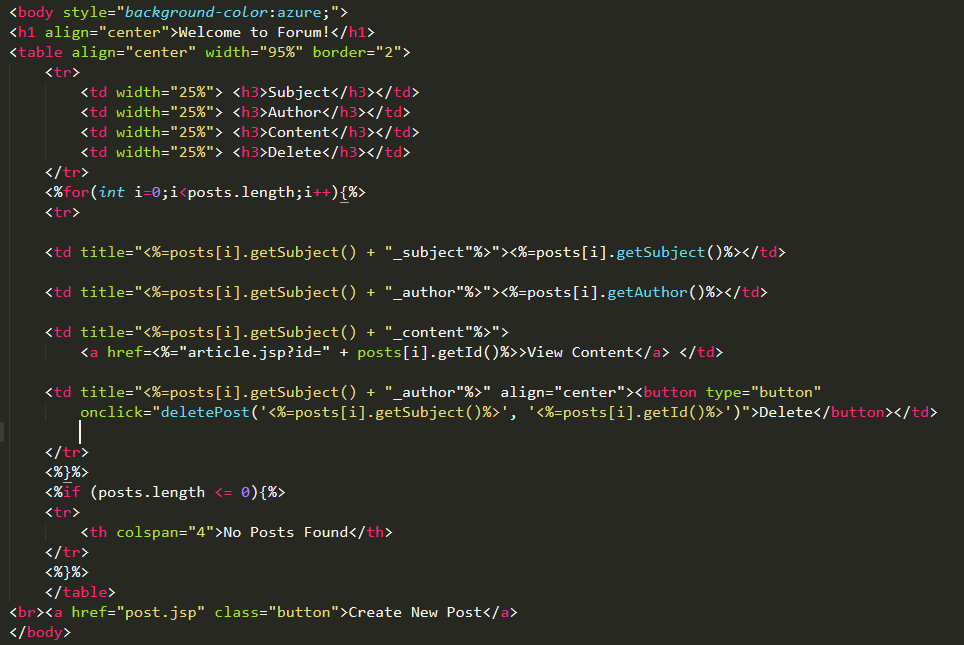
\includegraphics[width=0.5\textwidth]{code1.png}}
\caption{Sample page from application given to participants}
\label{code1}
\end{figure}

We recruited programmers with Java experience from Github
to participate in the study. We used Github to recruit participants rather than recruiting participants from our university or local software development firms, to get a more diverse sample of programmers. This is a widely accepted and used method among researchers to recruit participants for developer studies \cite{acar, acargit}. Furthermore, recruiting participants from Github helps to get participants with more experience in software development, which improves the ecological validity of the study \cite{acargit}. We extracted publicly available email addresses of Java developers with significant contributions to Java projects and sent emails inviting them to participate in our study. We offered them with a \$15 Amazon gift voucher as a token of appreciation for the participation. In the invitation email, we included a link to sign up for the study. Furthermore, we informed them that participation is voluntary and participants can withdraw from the study at any time. Sign up form required participants to enter their name and
email address, which were required to send study material to
them. However, such personally identifiable information of
the participants were removed from the final data set which
we used for the analysis. 

We conducted 4 usability studies parallelly and recruited
participants to all 4 studies together. We sent 13000 invitations
to Java developers and 347 developers signed up for the
study by completing the sign up form. Some emails we sent
were bounced and some developers requested to be removed
from our list, a request we honored. Furthermore, some people replied back to us saying that they are unable to
participate in the study. Once people signed up, we filtered
out those who did not have any software development experience
since our target sample for the study was software
developers. Furthermore, we filtered out participants with
no experience in using Java because if a participant faces issues
with programming language while completing the task,
we may not be able to clearly identify the usability issues of
the API s/he had come up with. Then we divided participants
who signed up into four studies we conducted based
on their demographics. We selected 51 programmers for the
ESAPI API study and sent study material for them. However, some of them informed that they are not able to complete the study and some of them dropped out without informing us. A total of 10 participants completed the study. 

Participants completed the task remotely on their own computers and we suggested them to complete the task in a time comfortable to them. We requested them to think-aloud \cite{thinkaloud} and record their screens with voice (so thinkaloud results will be recorded) while completing the task. By collecting participant think-aloud results, we expected to identify issues they experience by observing their thought process. Once a participant completed the task, s/he was asked to send his/her source code with the video recording to us through email. Participants spent an average of XXX minutes in completing the task. Then each participant had to complete the cognitive dimensions questionnaire \cite{wijaya} which we shared with them via Google forms.

Once we finished the data collection, source codes of solutions that participants developed were evaluated to see whether they have fixed the XSS vulnerability correctly. Application had 3 types of contexts (HTML, HTML Attribute and JavaScript) where participants had to protect using 3 different methods of the API (\textit{encodeForHTML(), encodeForHTMLAttribute(), encodeForJavaScript()}). We seperately evaluated whether participants had protected these elements of the web application successfully.

Then analysis of video recordings and questionnaire responses were done manually by one analyst. We used manual analysis since our data set was small \cite{manual}. Questionnaire answers were analysed prior to analysing videos and identified usability issues that exist in OWASP ESAPI from questionnaire responses. After analysing questionnaire answers, recordings were analysed to identify the usability issues that each participant encountered. For identifying usability issues from the screen recording data, user experience was evaluated by tracking the resources used, events where the participant showed surprise, events where participant had to make difficult choices, context switches, misconceptions, difficulties faced, mistakes made, requested features and time taken for tasks. Cognitive Dimensions Framework \cite{wijaya} was used as a guidance in the analysis of both questionnaire responses and recordings. Usability issues reporting format introduced by Lavery et al. \cite{lavery1997comparison} was used to report issues. Finally, video recordings were analysed to identify how usability issues that were identified, affected the participants for securely completing the task. Special attention was given to decisions made by participants that caused to reduce the security of programmes they developed.

\section{Study Results}

For the ease of presentation, we labeled participants with labels P1, P2,.., P10. They will be referred with this label from here onward. Statements made by participants that are presented in this section were not corrected for any grammatical errors and are presented as those were stated.

\subsection{Security of the Developed Programmes}

Table \ref{result} shows the security of application each participant developed. Furthermore, it shows which components of the web application they successfully secured and which components they failed to secure.

\begin{table}[htbp]
\caption[]{Security of Each Participant's Programme}
\begin{center}
\begin{adjustbox}{width=0.5\textwidth}
\begin{tabular}{|p{0.2\linewidth}| >{\centering\arraybackslash}p{0.2\linewidth}| >{\centering\arraybackslash}p{0.2\linewidth}| >{\centering\arraybackslash}p{0.2\linewidth}| >{\centering\arraybackslash}p{0.2\linewidth}|}
\hline
\textbf{Participant ID}&\textbf{Overall Security of the Aplication} & \textbf{Correctly Encoded HTML Content}  &\textbf{Correctly Encoded HTML Attribute Content} &\textbf{Correctly Encoded Javascript Content} \\

\hline
P1 & \cmark &\cmark &\cmark &\cmark \\
\hline
P2 & \xmark &\cmark &\xmark &\xmark \\
\hline
P3 & \xmark &\multicolumn{3}{c|}{Encoded input with encodeForHTML()} \\
\hline
P4 & \cmark &\cmark &\cmark &\cmark \\
\hline
P5 & \xmark &\multicolumn{3}{c|}{Encoded input with encodeForHTML() } \\
\hline
P6 & \xmark &\cmark &\cmark &\xmark \\
\hline
P7 & \xmark &\cmark &\xmark &\cmark \\
\hline
P8 &\xmark &\multicolumn{3}{c|}{Encoded input with encodeForHTML()} \\
\hline
P9 & \xmark &\multicolumn{3}{c|}{Encoded input with encodeForHTML()} \\
\hline
P10 & \xmark &\multicolumn{3}{c|}{Encoded input with encodeForHTML()} \\
\hline
\end{tabular}
\label{result}
\end{adjustbox}
\end{center}
\end{table}

We observed 3 main types of errors that participants did that resulted in them failing to secure the application.

\begin{enumerate}
\item Participants failed to identify all the places in the source code that contained XSS vulnerability and hence fixed the code partially (P2, P7).
\item Participants used wrong encoding method to encode data. For example, used \textit{encodeForHTML()} to encode data inside JavaScript (P2, P6).
\item Encoded input instead of output using one or two encoding methods. Mostly using \textit{encodeForHTML()} (P3, P5, P8, P9, P10).
\end{enumerate}

\subsection{Usability Issues of OWASP ESAPI}

From the study, we could identify a total of 16 usability issues that exist in OWASP ESAPI. Questionnaire responses revealed a total of 12 issues while video recording analysis revealed 12 issues of the API. Each participant had encountered an average of approximately 7 usability issues. Here onward, we extensively discuss each usability issue with the comments made by participants and what we observed.

Participants P2, P5, P6, P8 and P9 mentioned that there is too much information to read and learn in order to use the API to complete the task and fix XSS vulnerabilities. They mentioned that this makes it difficult for them to get the minimum understanding about the API that was required to use the API to fix the XSS vulnerabilities. Furthermore, they mentioned that it made it difficult for them to understand which part of the API to use in order to achieve the goal. P6 mentioned in his response to the questionnaire that ``\textit{Even though the guidelines, the cheatsheet, was actually well written , the page itself was kinda long-ish.}". One of the main resource provided from OWASP about using OWASP ESAPI to fix XSS vulnerabilities is the ``XSS Prevention Cheat sheet \cite{owasp10cheat}". Even though, it provided all the information required to use the API correctly to fix XSS vulnerabilities, most programmers did not follow it since it was too long. This made them refer to third party resources that provided partial solutions, which resulted in participants failing to successfully complete the task. This was elaborated by P3 as well where she mentioned that ``I did not even use the API documentation.There was a blog post with the required information, which was pretty much straight forward".

Results from all participants showed that it is difficult to use the API without previous knowledge on some computer security related areas. Results revealed that it was hard to use the API without a previous knowledge on attacks, XSS attacks, XSS mitigation techniques and input sanitization. We could identify that lack of security knowledge specially made it hard to test whether security vulnerability has been fixed properly, which resulted in participants deciding that they they have successfully fixed the XSS vulnerability. Some participants mentioned that they are not capable of testing what they developed due to their lack of security knowledge. P5 mentioned that ``\textit{It seems to me that output encoding untrusted data (which is done in one function call) sufficed, though I lack the knowledge to know if I've prevented all dangerous cases or not.}".

P1, P2 P3 and P8 mentioned that it was difficult to figure out how to achieve output encoding using the API. Some of them noted that programmer need to have a previous knowledge on what type of encoding is required for what type of elements. We observed these participants spent a notable amount of time for searching about things such as ``\textit{output encoding using OWASP ESAPI}". P2 highlighted this in his response to the questionnaire saying ``\textit{It was bit hard to grasp the idea of what output encoding and how we can achieve this with the API.}".

P3, P5, P6, P7, P8 and P9 faced difficulties while completing the task due to issues in OWASP ESAPI documentation. Their results revealed that,

\begin{itemize}
\item Official documentation is too lengthy.
\item Official documentation is not attractive for programmers.
\item Official documentation is difficult to understand.
\item Some documentation is outdated.
\end{itemize}

These issues resulted in programmers referring to unreliable third party resources to learn the API. P3 mentioned in her response to the questionnaire that ``\textit{I did not even use the API documentation. There was a blog-post with the required information which was pretty much straightforward}". Furthermore, above issues made programmers finding it difficult to use the API and learning process taking too much time. We observed many participants spent a considerable time to learn the API by going through documentation and other resources. P7 explained his experience with documentation saying ``\textit{I expected some documentation online - but after a few minutes I found that there is no up to date documentation available and I'd have to stick to JavaDoc and reading the sources}".

Another usability issues that participants encountered is the lack of examples. P2, P3, P6, P7 and P8 reported in their questionnaire responses as well as in their think aloud results that API lacks examples and proper getting started guide. P8 mentioned that ``\textit{In the document there are so many information but less usage examples. so it is hard to understand 1st time.}".  Participants mentioned that lack of examples made it difficult for them to learn the API and also made it difficult to know what classes and methods of the API to use when writing code. Participants suggested that including examples into documentation will give a better experience to programmers. P6 suggested that ``\textit{I would have liked a big h1 sign saying ``Example usage" for the APIs. Since I wasn't able to find examples as quick as I wished.}".

While completing the task, P5 and P10 found that Integrated Development Environment(IDE)'s suggestions are not working for the API. After entering method names, both these participants tried IDE suggestions to get an understanding about the required arguments for the method. Instead of providing useful suggestions, IDE showed parameter names such as arg0, arg1, etc. Participants mentioned that this made them to spent more time to learn the API and it made it difficult to use the API.

% if added before the last page, this command can help balancing columns
%\addtolength{\textheight}{-.2cm} 

%Bibliography 
\bibliographystyle{ieeetr}
\bibliography{sample}


\end{document}
